\section{Pianificazione}
Lo sviluppo del progetto è diviso nelle seguenti fasi consecutive.
\begin{enumerate}
	\item Analisi dei requisiti
	\item Progettazione architetturale
	\item Progettazione di dettaglio e codifica
	\item Validazione e collaudo
\end{enumerate}
Ogni fase è costituita da periodi, nei quali sono raggruppate le attività da svolgere.

\subsection{Analisi dei requisiti (dal 2020-10-22 al 2021-01-17)}

\subsubsection{Ruoli attivi}
\begin{itemize}
	\item Responsabile
	\item Amministratore
	\item Analista
	\item Verificatore
\end{itemize}

\subsubsection{Periodi e attività}

\paragraph{Primo periodo (dal 2020-10-22 al 2020-11-09)}
Questo periodo comincia con la costituzione del gruppo di progetto. Serve dunque a porre le basi per una comunicazione e collaborazione efficace ed efficiente. Vi si svolgono inoltre attività di ricerca superficiale sui capitolati.

\begin{itemize}
	\item Configurazione degli strumenti collaborativi basilari: comprende la scelta e la configurazione dei mezzi per la comunicazione e il lavoro collaborativo
	\item Analisi superficiale dei capitolati
	
\end{itemize}

\paragraph{Secondo Periodo (dal 2020-11-10 al 2020-12-13)}
Gli obiettivi raggiunti in questo periodo sono il consolidamento degli strumenti di collaborazione e l'approfondimento dei capitolati.
\begin{itemize}
	\item Configurazione del \glock{repository}: questa attività comprende la creazione di un repository per la condivisone e il versionamento dei prodotti, ma anche la sua configurazione per la verifica automatica della loro validità.
	\item Raccolta di informazioni dai seminari: stesura di appunti sui seminari, da poter facilmente consultare quando necessario.
	\item Studio dei progetti degli anni passati: questa attività ha il fine di individuare gli errori più comuni e, al contrario, le tecniche da prendere come esempio.
	\item Bozza dello studio di fattibilità
	\item Bozza delle norme di progetto
\end{itemize}

\paragraph{Terzo Periodo (dal 2020-12-14 al 2020-01-08)}
Questo periodo segue la scelta del capitolato da affrontare. E' dedicato alla sua analisi approfondita e alla stesura della documentazione. 
\begin{itemize}
	\item Stesura delle norme di progetto
	\item Stesura dello studio di fattibilità
	\item Stesura del piano di progetto
	\item Stesura del glossario
	\item Analisi dei requisiti e stesura dell'omonimo documento
	\item Stesura del piano di qualifica
	\item Verifica della documentazione
	\item Stesura della lettera di presentazione
\end{itemize}

\paragraph{Quarto Periodo (dal 2020-01-09 al 2020-01-17)}
Questo periodo è l'ultimo della fase di analisi dei requisiti. Si concentra quindi sulla preparazione dell'esposizione dei prodotti dei 3 periodi precedenti.
\begin{itemize}
	\item Preparazione dell'esposizione
	\item Verifica dell'esposizione
\end{itemize}


\begin{landscape}
	\begin{figure}[H]
		\centering
		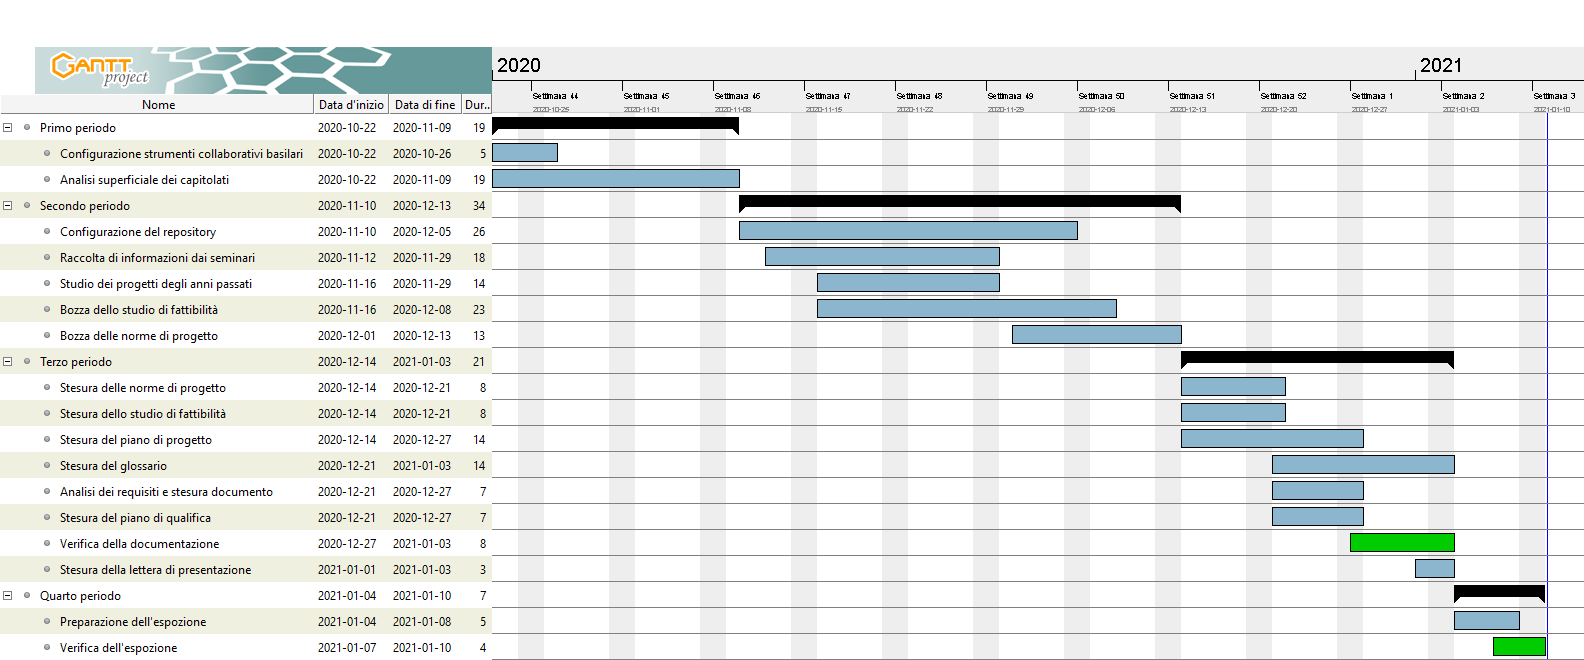
\includegraphics[width=\linewidth]{res/images/ganttFase1.png}
		\caption{Grafico di Gantt della fase di analisi dei requisiti}
		\label{fig:Gantt Analisi dei requisiti}
	\end{figure}
\end{landscape}

\subsection{Progettazione architetturale (dal 2021-01-18 al 2021-03-07)}

\subsubsection{Ruoli attivi}
\begin{itemize}
	\item Responsabile
	\item Amministratore
	\item Analista
	\item Progettista
	\item Verificatore
\end{itemize}

\subsubsection{Periodi e attività}

\paragraph{Primo Periodo (dal 2021-01-18 al 2021-01-23)}
\begin{itemize}
	\item Aggiornamento Norme di progetto
	\item Aggiornamento Piano di qualifica
	\item Aggiornamento Piano di progetto
	\item Verifica documentazione
\end{itemize}

\paragraph{Secondo Periodo (dal 2021-01-24 al 2021-02-16)}
\begin{itemize}
	\item Aggiornamento requisiti
	\item Ricerca
	\item Progettazione
	\item Verifica
\end{itemize}

\paragraph{Terzo Periodo (dal 2021-02-17 al 2021-02-25)}
\begin{itemize}
	\item Progettazione Proof of concept
	\item Codifica Proof of concept
	\item Verifica Proof of Concept
\end{itemize}

\paragraph{Quarto Periodo (dal 2021-02-26 al 2021-03-07)}
\begin{itemize}
	\item Stesura Lettera di presentazione
	\item Verifica Lettera di presentazione
	\item Preparazione presentazione
	\item Verifica della presentazione
\end{itemize}

\begin{landscape}
	\begin{figure}[H]
		\centering
		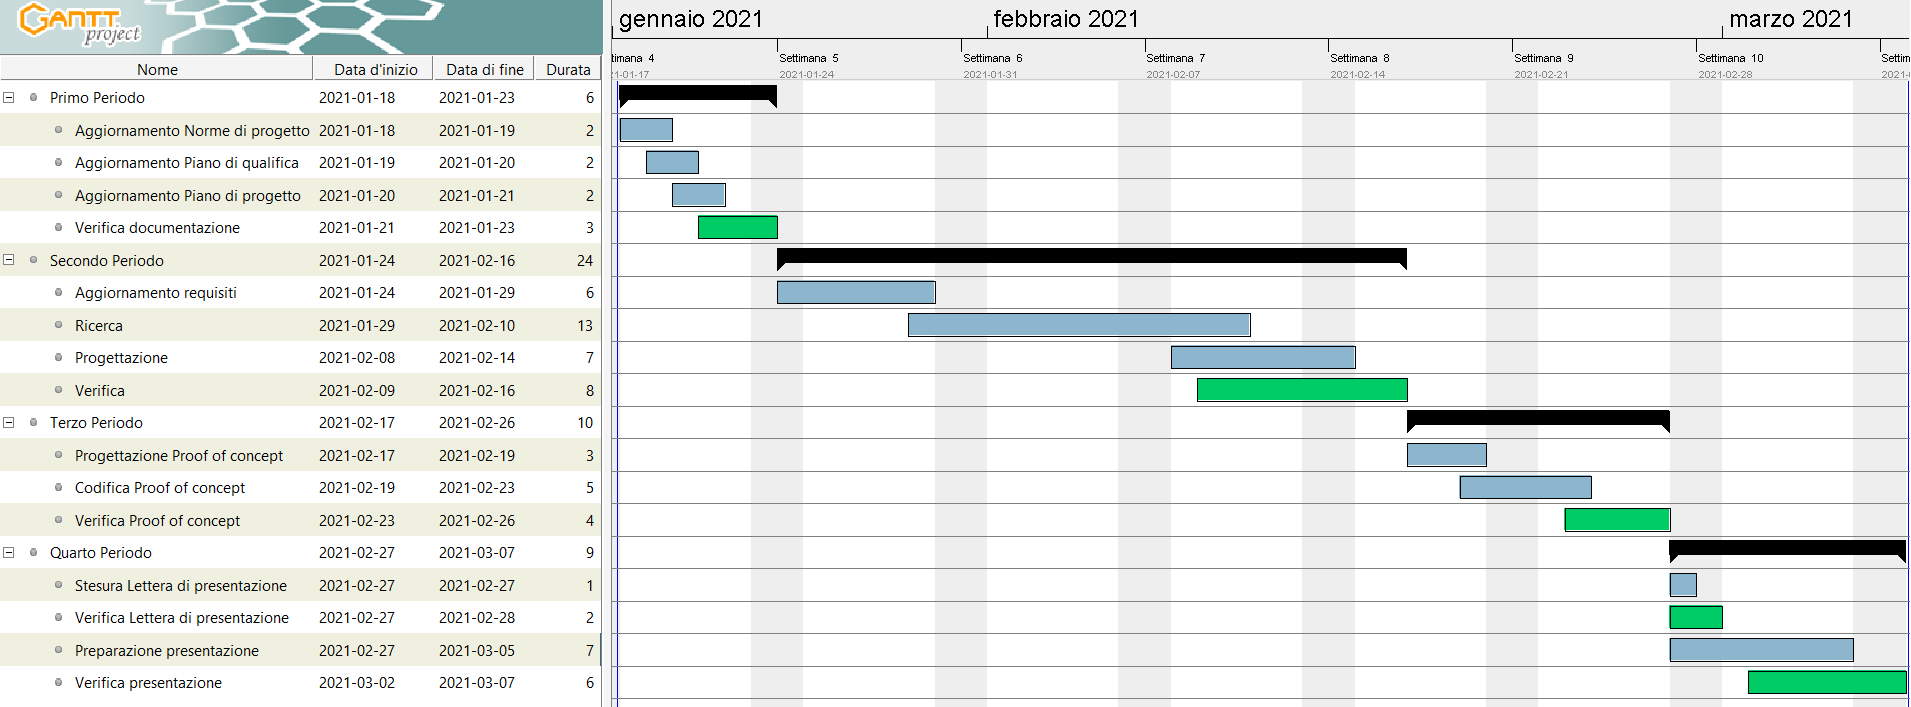
\includegraphics[width=\linewidth]{res/images/ganttFase2.png}
		\caption{Grafico di Gantt della fase di Progettazione architetturale}
		\label{fig:Gantt Analisi dei requisiti}
	\end{figure}
\end{landscape}

\subsection{Progettazione di dettaglio e codifica (dal 2021-03-01 al 2021-04-08)}

\subsubsection{Ruoli attivi}
\begin{itemize}
	\item Responsabile
	\item Amministratore
	\item Analista
	\item Progettista
	\item Programmatore
	\item Verificatore
\end{itemize}

\subsubsection{Periodi e attività}

\paragraph{Primo Periodo (dal 2021-04-02 al 2021-01-23)}
\begin{itemize}
	\item Aggiornamento Norme di progetto
	\item Aggiornamento Piano di qualifica
	\item Aggiornamento Piano di progetto
	\item Verifica documentazione
\end{itemize}

\paragraph{Secondo Periodo (dal 2021-01-24 al 2021-02-16)}
\begin{itemize}
	\item Collaudo
\end{itemize}

\paragraph{Terzo Periodo (dal 2021-02-17 al 2021-05-02)}
\begin{itemize}
	\item Stesura Lettera di presentazione
	\item Verifica Lettera di presentazione
	\item Preparazione presentazione
	\item Verifica della presentazione
\end{itemize}

\subsection{Validazione e collaudo (dal 2021-04-09 al 2021-05-09)}

\subsubsection{Ruoli attivi}
\begin{itemize}
	\item Responsabile
	\item Amministratore
	\item Progettista
	\item Programmatore
	\item Verificatore
\end{itemize}

\subsubsection{Periodi e attività}

\paragraph{Primo Periodo (dal 2021-04-09 al 2021-04-15)}
\begin{itemize}
	\item Aggiornamento Norme di progetto
	\item Aggiornamento Piano di qualifica
	\item Aggiornamento Piano di progetto
	\item Verifica documentazione
\end{itemize}

\paragraph{Secondo Periodo (dal 2021-01-24 al 2021-02-16)}
\begin{itemize}
	\item Collaudo
\end{itemize}

\paragraph{Terzo Periodo (dal 2021-05-01 al 2021-05-09)}
\begin{itemize}
	\item Stesura Lettera di presentazione
	\item Verifica Lettera di presentazione
	\item Preparazione presentazione
	\item Verifica della presentazione
\end{itemize}

